\subsubsection{Embedded Systems Modeling and Deep Compositionality (Krogh, Tomlin, Sastry)}
                 
                 \emph{Verification of Stochastic Hybrid Systems}
                 %    \newline \small{ Graduate Student: Maryam Kamgarpour}

                 \begin{figure}[!t]
                   \begin{center}
                     \begin{subfigmatrix}{2}% number of columns
                       \subfigure[Reach-Avoid problem]{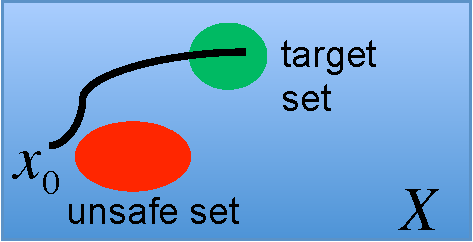
\includegraphics{img/reachavoidsets.pdf}}                
                       \subfigure[Probabilistic backward reach-avoid set]{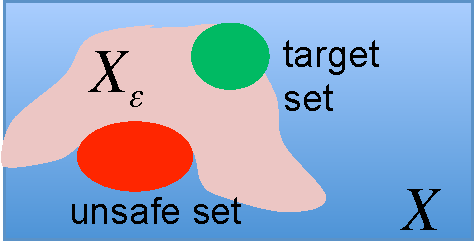
\includegraphics{img/reachavoidoptimal.pdf}}
                     \end{subfigmatrix}   
                     \caption{Reach-avoid problem for stochastic hybrid systems}
                     \label{fig:reach_avoid_problem}
                   \end{center}
                 \end{figure}

         

                 We consider a general hybrid modeling framework in
                 which we account for stochastic disturbances in
                 evolution of the continuous and discrete states. In
                 addition, we account for deterministic disturbances
                 in the model. The motivation is that while some
                 classes of uncertainty, such as those by nature, are
                 best modeled stochastically, some other classes of
                 uncertainty, such as those due to presence of agents
                 with competing objectives, are best modeled in a
                 deterministic worst-case approach. For example, in a
                 collision avoidance scenario between two aircraft, on
                 the one hand, wind affects the dynamics of aircraft
                 and uncertainties in wind forecast and measurement
                 may be best accounted for through a stochastic
                 framework. On the other hand, in the absence of
                 communication between the aircraft, from the
                 perspective of each aircraft, the trajectory must be
                 safe in the worst-case performance of the other
                 aircraft. Hence, a robust approach should be
                 considered.

                 The reach-avoid objective in the setting of the
                 stochastic hybrid system with two players becomes a
                 stochastic game in which the objective of player 1
                 (the control) is to steer the hybrid system state
                 into a desired target set, while avoiding a set of
                 unsafe states, as shown in Figure
                 \ref{fig:reach_avoid_problem}(a).  On the other hand,
                 the objective of player 2 (the adversary) is to
                 either steer the state into the unsafe set or prevent
                 it from reaching the target set.

                 Mathematically, the problem is stated as follows: Let
                 $X$ denote the hybrid state space. Suppose that Borel
                 sets $G, S \in \mathcal{B}(X)$ are given as the
                 desired target set and safe set, respectively, with
                 $G \subseteq S$.  Then the probability that the state
                 trajectory $(x_0, x_1, \dots, x_N)$ reaches $G$ while
                 staying inside $S$ under fixed choices of player 1
                 policy $\mu \in \mathcal{M}_a$ and player 2 strategy
                 $\gamma \in \Gamma_d$ is \cite{kamgar2011cdc}:

                 \begin{align*}
                   \label{eq:reachavoid_prob_expectation}
                   r_{x_0}^{\mu, \gamma}&(G,S) = E^{\mu,\gamma}_{x_0} \left[ \mathbf{1}_G(x_0) + \sum^{N}_{j=1}\left(\prod^{j-1}_{i=0}\mathbf{1}_{S\setminus G}(x_i)\right)\mathbf{1}_G(x_j)\right],
                 \end{align*}
                 where $E^{\mu,\gamma}_{x_0}$ denotes the expectation
                 with respect to the probability measure
                 $P_{x_0}^{\mu, \gamma}$ induced by the initial
                 condition, $x_0 \in X$, and the players'
                 strategies. The admissible control spaces consist of
                 the set of Markov policies and strategies, denoted by
                 $\mathcal{M}_a$, $\Gamma_d$, for the control and
                 adversary, respectively.

                 Define the worst-case reach-avoid probability under a
                 choice of Markov policy $\mu$ as $r_{x_0}^\mu(G,S) =
                 \inf_{\gamma \in \Gamma_d} r_{x_0}^{\mu,
                   \gamma}(G,S).$ Our objective is to maximize this
                 worst-case probability over the set of Markov
                 policies. Thus, we need to compute the maxmin value
                 function $r_{x_0}^*(G,S) := \sup_{\mu \in
                   \mathcal{M}_a} r_{x_0}^\mu(G,S)$, and find a maxmin
                 policy $\mu^* \in \mathcal{M}_a$, such that
                 $r_{x_0}^*(G,S) = r_{x_0}^{\mu^*}(G,S)$, $\forall x_0
                 \in X$.

                 We have developed a dynamic programming algorithm for
                 maximizing the reach-avoid probability and for
                 synthesizing a control law that achieves this
                 probability. In addition, from this algorithm we can
                 find the set of initial conditions $X_\epsilon$ for
                 which the reach-avoid probability is above
                 $(1-\epsilon)$, $\forall \epsilon \in [0,1]$, under
                 the worst-case adversary behavior, as shown in Figure
                 \ref{fig:reach_avoid_problem}(b).

                 The algorithm has been applied to several robust
                 motion planning problems including a quadrotor
                 helicopter tracking a ground vehicle and aircraft
                 conflict detection and resolution scenarios
                 \cite{kamgar2011cdc}.

                 \emph{Aircraft Conflict Detection}

                 The scenario involves two aircraft with possibly
                 intersecting nominal trajectories. From the
                 perspective of the first aircraft, the task is to
                 detect the possibility of conflict given current
                 position of another aircraft, and design a collision
                 avoidance trajectory in case potential conflict is
                 detected. Motivated by wind influence on aircraft
                 trajectories and on accuracy of conflict detection,
                 we consider wind with a deterministic component,
                 known through forecast or measurements, and a
                 stochastic component to capture its
                 uncertainties. Based on geostatistics analysis of
                 wind data, the stochastic wind component is modeled
                 as a time dependent random field over the $2D$
                 airspace.

                 A conflict is defined if aircraft get closer than a
                 critical distance of $R_c$. Hence, the safe set in
                 $2D$ can be defined in relative coordinates as: $S =
                 \{ (x^1,x^2) \in \mathbb{R}^2 \; s. t. \; \|
                 (x^1,x^2) \|_2 \geq R_c \}$.For conflict detection,
                 we assume that the current position of each aircraft
                 is available, for example through Automatic Dependent
                 Surveillance-Broadcast (ADS-B) network. For the
                 conflict resolution, we assume that the control of
                 the two aircraft are decentralized. Furthermore, in
                 the absence of further information on the decision
                 algorithms, each aircraft assumes that the other
                 aircraft could potentially make choices that endanger
                 safety.


                 The aircraft kinematics is modeled as a unicycle. The
                 input of each aircraft is its heading angle
                 rate. Motivated by discrete maneuvers used in air
                 traffic, we assume at any given time, each aircraft
                 can choose to be in one of three flight maneuvers:
                 straight, right turn, or left turn.

                 \begin{figure}[!t]
                   \begin{center}
                     \begin{subfigmatrix}{2}
                       \subfigure[Maxmin probability of safety]{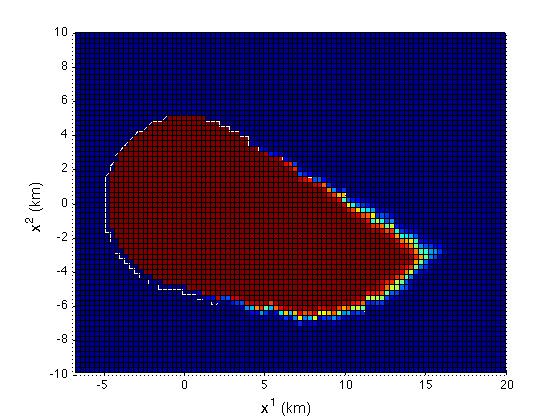
\includegraphics{img/pminmax_3pi4}}                
                       \subfigure[Deterministic reachable set]{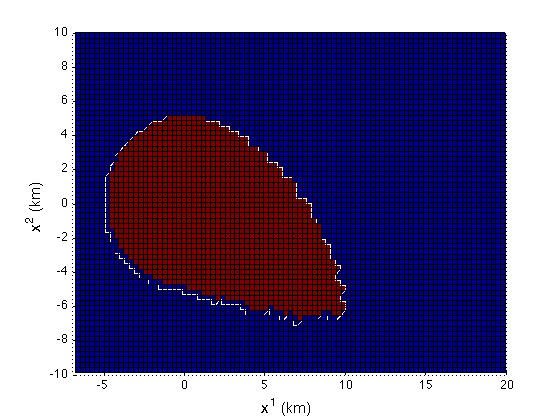
\includegraphics{img/deterministic_3pi4}}
                     \end{subfigmatrix}
                     \caption{Collision detection in probabilistic and deterministic settings}
                     \label{fig:prob_collision1}
                   \end{center}
                 \end{figure}

                 The maxmin probability of safety over a horizon of
                 $2.5$ minutes and with aircraft speed of $5$ km per
                 minute, is computed based on our proposed dynamic
                 programming algorithm. Figure
                 \ref{fig:prob_collision1}(a) illustrates this
                 probability for the set of initial conditions with
                 relative heading of $\frac{3\pi}{4}$ radians. The
                 interpretation of this probability map is as
                 follows. Consider an initial condition of $(10.55
                 \text{ km}, -6.85 \text{ km},\frac{3\pi}{4} \text{
                   rad})$. From the value function we obtain the
                 maxmin probability of safety to be $99 \%$.  This
                 means that if aircraft 1 selects flight maneuvers
                 according to the maxmin policy $\mu^*$ and aircraft 2
                 selects any maneuvers within the set of Markov
                 strategies, the probability of collision would remain
                 at most $1 \%$. For comparison, the result of
                 deterministic computation, in which wind influence is
                 ignored, is shown in Figure
                 \ref{fig:prob_collision1}(b). In this case, any
                 initial condition is characterized as being safe or
                 not.

                 \emph{Uncertain Safe and Target Sets}

                 \begin{figure}[!t]
                   \begin{center}
                     \begin{subfigmatrix}{2}
                       \subfigure[VIL measurements from forecast]{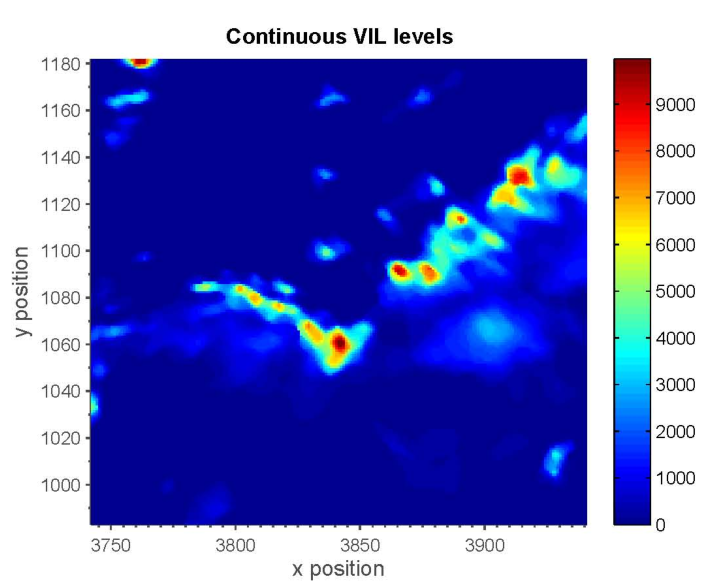
\includegraphics{img/VILcontinuous}}                
                       \subfigure[No-fly zones based on forecast]{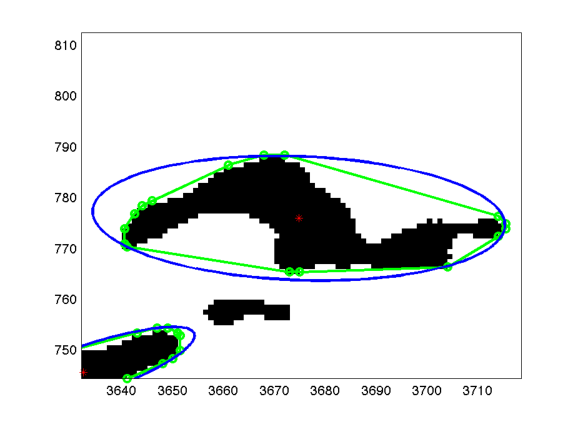
\includegraphics{img/VILenclosed}}
                     \end{subfigmatrix}
                     \caption{Forecast data for Vertically Integrated Liquid level}
                     \label{fig:vil}
                   \end{center}
                 \end{figure}

                 It has been shown that high values of Vertically
                 Integrated Liquid (VIL) level indicate storm
                 precipitation and regions with high VIL levels should
                 be avoided by pilots. We have used MIT Lincoln lab
                 forecast of VIL data over a gridded United States
                 airspace to characterize obstacles in aircraft
                 flight. Figure \ref{fig:vil}(a) shows the forecast
                 data for 01/07/2009 near gulf coast of Florida, while
                 Figure \ref{fig:vil}(b) shows the minimum-volume
                 geometric shapes enclosing the regions with high VIL
                 values in order to use them in an optimization
                 algorithm. In \cite{maryam2011ifac} we used a
                 deterministic hybrid optimal control approach to find
                 fuel efficient aircraft trajectories which avoid
                 these hazardous regions. Also, based on the actual
                 and forecast data, we modeled the storm movement over
                 time and formulated a receding horizon nonlinear
                 program to design conflict-free aircraft trajectories
                 which avoid moving storms
                 \cite{kamgarpour2010cdc}. Clearly, the actual weather
                 deviates from the forecast, specially, with
                 increasing forecast horizon. To account for such
                 environmental uncertainties, we introduced a
                 parametrized set-valued stochastic process model for
                 the stochastic target and safe sets in the
                 reach-avoid problem. In
                 \cite{summers2011stochasticset} we showed that the
                 verification and control synthesis for stochastic
                 hybrid systems with stochastic sets can be addressed
                 by an appropriate dynamic programming algorithm.

                 We used our methodology to optimize the probability
                 that the aircraft attains a rectangular region around
                 a waypoint shown in Figure
                 \ref{fig:prob_decoupled}(b), while avoiding the
                 stochastic unsafe sets, representing the storm
                 locations, over the $30$ minute horizon and to
                 synthesize an optimal Markov policy that achieves
                 this probability. The optimal value function, is
                 shown in Figure \ref{fig:prob_decoupled}(a) for all
                 initial positions $(x_0,y_0)$ in $2D$ with an initial
                 heading angle of $\psi_0 = -0.785$ radians. An
                 example execution of the process is shown in Figure
                 \ref{fig:prob_decoupled}(b).
                 \begin{figure}
                   \begin{center}
                     \begin{subfigmatrix}{2}
                       \subfigure[Probability map for $\psi_0 =-0.785$]{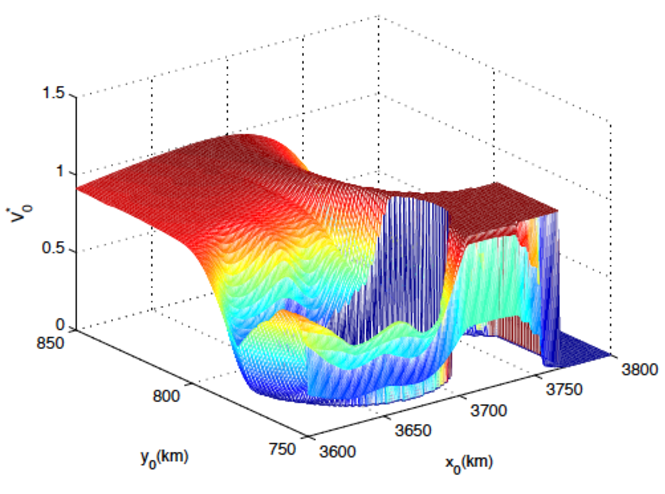
\includegraphics{img/Ch4ProbDecoupled}}                
                       \subfigure[Maximally safe trajectory]{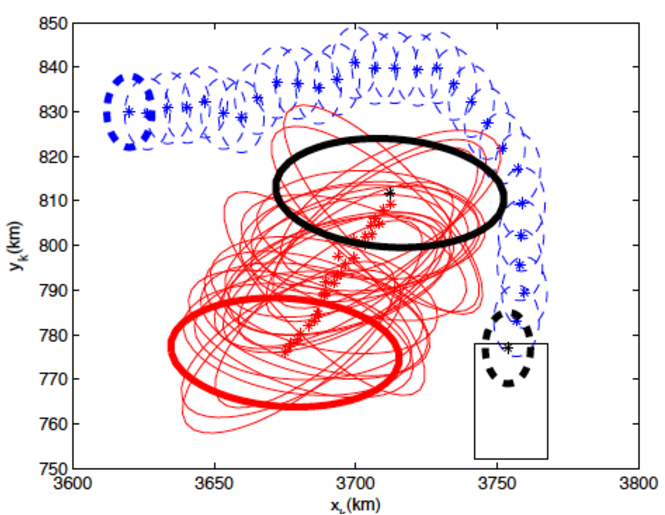
\includegraphics{img/Ch4PathDecoupled}}
                     \end{subfigmatrix}
                     \caption{Aircraft trajectory planning in stochastic environment}
                     \label{fig:prob_decoupled}
                   \end{center}
                 \end{figure}


